\documentclass{article}
\usepackage[utf8]{inputenc}
\usepackage[spanish]{babel}
\usepackage{listings}
\usepackage{graphicx}
\graphicspath{ {images/} }
\usepackage{cite}

\begin{document}

\begin{titlepage}
    \begin{center}
        \vspace*{1cm}
            
        \Huge
        \textbf{Proyecto De Investigación}
            
        \vspace{0.5cm}
        \LARGE
        Taller Memoria
            
        \vspace{1.5cm}
            
        \textbf{Andrés Felipe Rendón Villada}
            
        \vfill
            
        \vspace{0.8cm}
            
        \Large
        Despartamento de Ingeniería Electrónica y Telecomunicaciones\\
        Universidad de Antioquia\\
        Medellín\\
        Septiembre de 2020
            
    \end{center}
\end{titlepage}

\tableofcontents

\section{Sección introductoria}
Los desarrollos tecnológicos que se han obtenido a lo largo de la historia, han desempeñado un papel muy importante en nuestras vidas, pues nos han facilitado en gran medida el desarrollo de muchas actividades. Por esta razón en este trabajo nos centraremos en uno de los avances tecnológicos mas importantes del siglo XX, el computador.
\newline
A continuación procederemos con el estudio de uno de los componentes que integran el hardware, la "memoria". 

\section{Preguntas} \label{contenido}

\subsection{¿Qué es la memoria?} \label{contenido}
La memoria es un circuito electrónico que está compuesto por un conjunto de chips, ésta se encuentra presente en el hardware de nuestros dispositivos tecnológicos (como: PC, celulares, electrodomésticos, etc.). Su función consiste en guardar la información que van a ejecutar dichos dispositivos (por ejemplo, los programas que contienen las instrucciones para que funcione el dispositivo).
\newline
La memoria funciona mediante señales eléctricas, que comúnmente se suele denominar binario (0 cuando exista ausencia de voltaje y 1 para indicar que hay voltaje). Su capacidad se mide en byte (que son la unión de 8 bits). La memoria (en este caso la de un computador). " Guarda de forma temporal la información que se obtiene de ejecutar las instrucciones que ingresa el usuario mediante los periféricos de entrada de la máquina (estas instrucciones se traducen a código binario, es decir, cadenas de ceros y unos que es lo que entiende el procesador)".\cite{Quiroga}.
\newline
"La memoria está en constante comunicación con la CPU quien recibe las instrucciones y datos de entrada que previamente fueron guardados en la memoria (todas la modificaciones o manipulación de la información no se efectúan directamente sobre la información contenida en el disco duro, si no en una copia que se encuentra en ejecución en la memoria). La gran ventaja que posee la memoria frente a otros dispositivos como el disco duro, es que la memoria tiene mayor velocidad para procesar la información".\cite{Guia}.

\subsection{Tipos de memoria y descripcion de cada una de ellas}
\textbf{Memoria RAM:}
Memoria de acceso aleatorio.
\newline
\newline
"La memoria RAM es la memoria principal de un dispositivo donde se almacena programas y datos informativos. Las siglas RAM significan “Random Access Memory” traducido al español es “Memoria de Acceso Aleatorio”.
La memoria RAM es conocida como memoria volátil lo cual quiere decir que los datos no se guardan de manera permanente, es por ello, que cuando deja de existir una fuente de energía en el dispositivo la información se pierde. Asimismo, la memoria RAM puede ser reescrita y leída constantemente."\cite{RAM} 
\newline
\newline
A continuación se presenta la imagen de una memoria RAM (\ref{fig:memoria-RAM})
\begin{figure}[h]
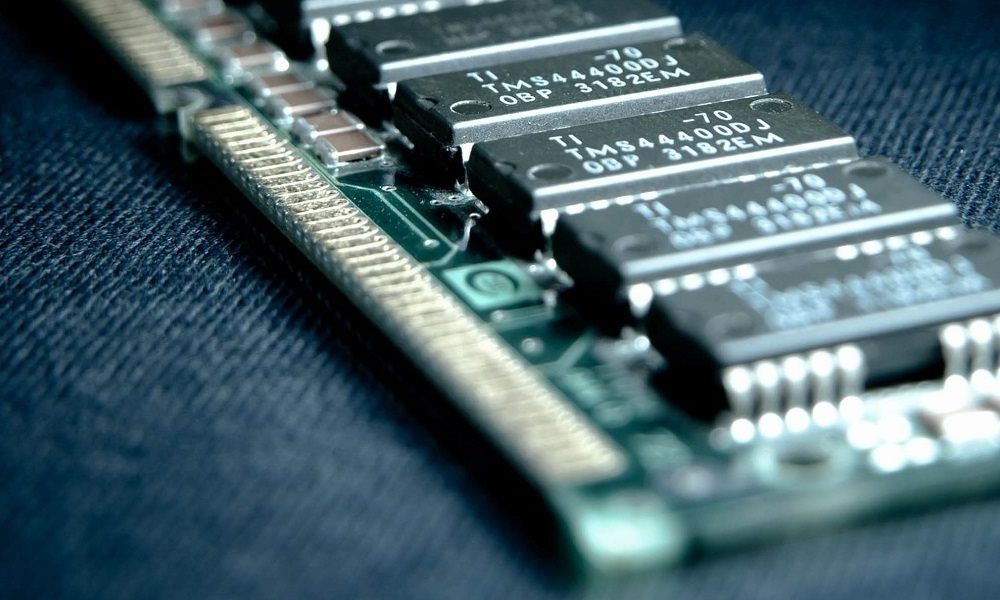
\includegraphics[width=4cm]{memoria-RAM.jpg}\centering
\caption{Memoria RAM}
\label{fig:memoria-RAM}
\end{figure}
\newline
\textbf{Memoria ROM:} Memoria de solo lectura.
\newline
\newline
"La memoria ROM es el medio de almacenamiento de programas o datos que permiten el buen funcionamiento de los ordenadores o dispositivos electrónicos a través de la lectura de la información sin que pueda ser destruida o reprogramable. El significado de memoria ROM es “Read Only Memory” traducido al español “Memoria de solo lectura.”
\newline
La memoria ROM es conocida como memoria no volátil ya que la información contenida en ella no es borrable al apagar el dispositivo electrónico.
\newline
La memoria ROM se encuentra instalada en la tarjeta madre “motherboard” lugar donde se encuentra la información básica del equipo, llamada “BIOS.”"\cite{ROM}
\newline
\newline
A continuación se presenta la imagen de una memoria ROM (\ref{fig:memoria-ROM})
\begin{figure}[h]
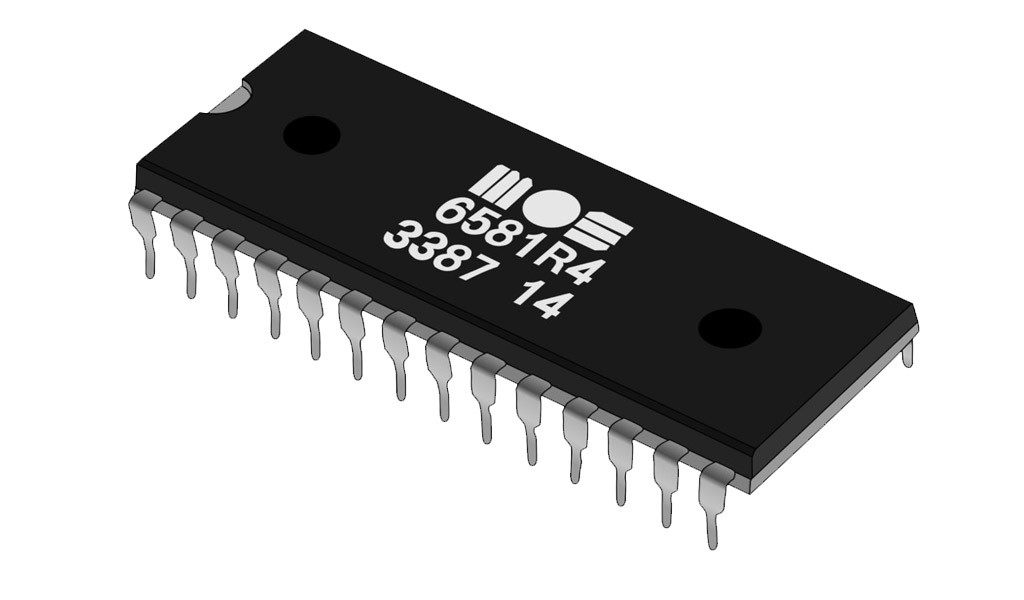
\includegraphics[width=4cm]{memoria-ROM.jpg}\centering
\caption{Memoria ROM}
\label{fig:memoria-ROM}
\end{figure}
\newline 
\newline 
\textbf{Memoria cache}
\newline
\newline
"Se conoce como memoria caché o memoria de acceso rápido a uno de los recursos con los que cuenta una CPU (Central Processing Unit, o sea, Unidad Central de Procesamiento) para almacenar temporalmente los datos recientemente procesados en un búfer especial, es decir, en una memoria auxiliar.
\newline
La memoria caché opera de modo similar a la Memoria Principal del CPU, pero con mayor velocidad a pesar de ser de mucho menor tamaño. Su eficacia provee al microprocesador de tiempo extra para acceder a los datos más frecuentemente utilizados, sin tener que rastrearlos a su lugar de origen cada vez que sean necesarios."\cite{Cache}
\newline
\newline
\textbf{Memoria RAM Dinámica (Dynamic RAM)}
\newline
\newline
"Sus siglas provienen del nombre inglés Dynamic Random Access Memory, es decir, Memoria Dinámica de Acceso Aleatorio. También se conoce como una RAM dinámica. Este tipo de memoria fue ideada en los laboratorios de la reconocida compañía IBM a mediados de 1960.
\newline
La memoria DRAM se trata de una tecnología que está fabricada en condensadores. Lo que caracteriza a esta memoria es que, al ser dinámica, la misma pierde su carga progresivamente, por lo que necesitan de circuitos dinámicos de refresco cada cierta cantidad de tiempo.
\newline
En este sentido, un aspecto fundamental de cómo funciona la memoria DRAM es que se trata de una memoria volátil. Lo anterior quiere decir, que la misma pierde sus datos una vez que es desconectada de su fuente de energía."\cite{DRAM}
\newline
\newline
A continuación se presenta la imagen de una memoria DRAM
(\ref{fig:memoria-DRAM})
\begin{figure}[h]
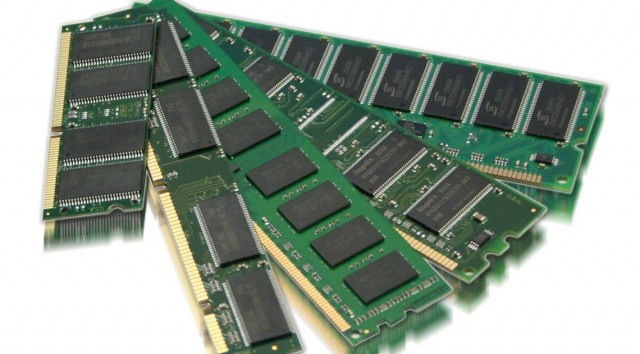
\includegraphics[width=4cm]{dram.jpg}\centering
\caption{Memoria DRAM}
\label{fig:memoria-DRAM}
\end{figure}
\newline
\newline
\textbf{Memoria flash}
Es un dispositivo electronico, que permite realizar lectura y escritura de información. y que al suspender la fuente de alimentacion esta sigue conservando la informacion que se habia guardado previamente en ella.\cite{flash}.
\newline
\newline
A continuación se presenta la imagen de una memoria flash
(\ref{fig:memoria-flash})
\begin{figure}[h]
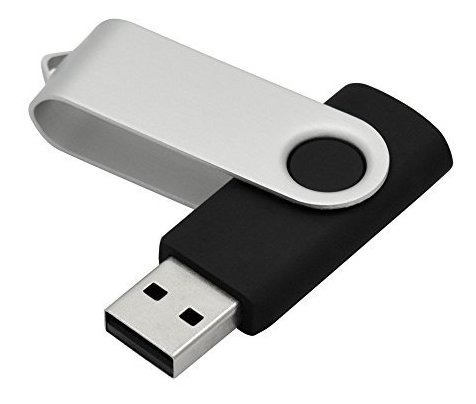
\includegraphics[width=4cm]{memoria-flash.jpg}\centering
\caption{Memoria flash}
\label{fig:memoria-flash}
\end{figure}
\newline
\newline
\

\subsection{¿Como se gestiona la memoria en el computador?}
En nuestro computador hay presentes distintos tipos de memorias, por ejemplo: la memoria ROM (en la cual se encuentra la BIOS de nuestra maquina). una vez encendemos nuestro computador la memoria ROM se encarga de realizar el chequeo de los componentes de nuestro dispositivo, una vez completado este chequeo, accede a la sección del disco duro donde esta instalado el sistema operativo y carga las instrucciones del sistema operativo en la memoria RAM, la cual  trabaja en conjunto con el microprocesador este recibe la información de la memoria RAM para ejecutar los procesos previamente definidos , una vez inicie el sistema y se ejecute algun programa, este sera cargado en la memoria para que el microprocesador tenga acceso inmediato a esta informacion. Pues la memoria es mas rápida que el disco duro, pero esta memoria (la RAM) es volátil por lo que al apagar el dispositivo toda la información que se encuentra en la memoria se borrara una vez se corte el suministro electrico.\cite{Guia},\cite{Gestion}
\newline
\subsection{¿Qué hace que una memoria sea más rápida que otra? ¿Por qué esto es importante?}

Hay varios factores que podriamos tener encuenta para analizar la rapidez de una memoria:
\newline
1. la latencia: mide la cantidad de tiempo que se tarda en obtener de la memoria cada bit de información, o sea el tiempo que pasa desde que el controlador de memoria pide en nombre del microprocesador
una serie de datos y dichos datos son obtenidos.\cite{Guia}
\newline
2,La aquitectura de la memoria: dependiendo de los componentes con los que se fabricó la memoria, por ejemplo: la memoria RAM tiene chips integrados en la placa (circuito impreso), mientras que el disco duro esta compuesto por uno o mas discos. Pero la memoria aun que no puede guardar datos de forma temporal (cosa que el disco duro si puede hacer), esta puede acceder a la información mucho mas rápido que el disco duro  debido a que la información no se guarda de forma secuencial en la memoria (a diferencia del disco duro que graba de forma magnetica la informacion en los discos o platos), por lo que sin importar la ubicación de la información en las "celdas" de la memoria, se podra acceder de forma rápida a la información que se desea, mientras que en el disco duro se tendria que recorrer todo el disco hasta encontrar la información.\cite{Quiroga}
\newline
3.Su utilizadad: dependiendo de la función que valla a desempeñar la memoria podria tener mas velocidad respecto a otras por ejemplo la memoria cache es mas rapida que la RAM, pero la RAM es mas rapida que memoria virual quien es mas rapida que el discoduro.
\newline
¿por que es importante?, es importante por que se puede acceder a la información o ejecutar algun proceseo de que el tiempo de espera para obtener el resultado esperado sea mucho menor.

\section{Conclusión} \label{conclulsion}

1. En los computadores existen diferentes tipos de memorias ademas de la RAM y cada una cumple una funcion importante para el correcto funcionamiento del dispositivo (como la Memoria ROM que realiza el chequeo de los componentes del hardware del computador y ademas cuenta con la Bios del Computador).
\newline
\newline
2. El almacenamiento en la memoria RAM , se realiza por medio de "Celdas" , las cuales tienen una respectiva dirección para almacener bits de información
\newline
\newline
3. La memoria RAM a diferencia del disco duro o de una memoria flash , es una memoria volátil es decir , que cuando se corte el suministro electrico la información que este cargada en la memoria se borrara
\bibliographystyle{IEEEtran}
\bibliography{references}

\end{document}
